\documentclass[11pt,letterpaper]{report}
\usepackage{listings} % Allow listing of source codes
\usepackage{tikz}
\usetikzlibrary{shapes, arrows, shadows}
\usepackage{graphicx}   % Required to use pictures
\usepackage{cite}
\usepackage{url}  % \url command for bibliography entries
\usepackage{setspace}   % Control line spacing
\lstset{numbers=left,
numberstyle=\tiny,basicstyle=\small,
tabsize=2,breaklines,showstringspaces=false,frame=tB}
\lstset{literate=
{ö}{{\"o}}1
{ä}{{\"a}}1
{ü}{{\"u}}1
{Ö}{{\"O}}1
{Ü}{{\"U}}1
{Ä}{{\"A}}1
{ß}{{\ss{}}}1}

\title{Schema Designing to Index Some Available Materials Related to Software Certification}
\author{
        \normalsize
        Ishwaree Argade
            \mbox{}\\ %
        \normalsize MEng(Computer Science)
         \mbox{} \\
       \normalsize Department of Computing and Software 
                \mbox{}\\ %
        \normalsize McMaster University 
        \mbox{} \\
        \date{\today} \\
}


\begin{document}
\maketitle

\begin{abstract}

Software Certification is the process of certifying the systems scoped to their software part. The report emphasizes on the task of indexing some available material around the various areas of software certification and thus explains the idea of software repository. However, it revolves around Challenge Problems, Course Modules and Certified Software Libraries and Tools which are the three areas related to Software Certification and also are the three components of the repository. The scope of the report is to design and implement schemas using XSDs to index some important information for the above three areas. The report starts with the introduction to the software certification and some approaches followed to perform software certification. It then describes the idea of software repository and the need for schema design to store the data in the repository. The schemas are implemented using XSDs. Thus, the latter chapters explain the process of schema design and present implementations followed by the corresponding XSLs for challenge problems, course modules, libraries and tools respectively. Further part provides an overview of testing process and a representative case study for challenge problem category.  
\end{abstract}

\setcounter{tocdepth}{2}
\tableofcontents

\chapter{Introduction}

Software Certification deals with the process of certifying a system containing some sort of software inside it but, restricting the certification process to the software aspect only \cite{seminar}. The certification process ensures the reliability and safety of the software system to be certified listing all the information necessary for its assessment. It encompasses wide range of formal, semi-formal and informal assurance techniques which includes even formal verification of safety policies, system simulation, testing and code reviews \cite{SCMS}. Thus, the certificates can have various types and certification process follow various mechanisms. 

Most popular approach for software certification is process based certification of systems. The process through which a software system is developed is evaluated rather than evaluating the final product. As many software certifiers find the evaluation of software process easier than evaluation of product itself, process based certification is widely used \cite{Lawford}. One reason for this is, it is not possible to test the final product entirely even with the help of huge number of test cases. Hence, the focus is given on certain supportive evidences which would guarantee the quality of the software systems. Secondly, it is difficult to determine the metrics/attributes essential in assessing the final software product, more emphasis is given on the software process instead \cite{Lawford}. Some examples of this approach like ISO 9000 and CMMI certify that the proper engineering methods and processes are followed to manufacture the product \cite{Voas}.

Though process based certification is a popular approach, it doesn't guarantee the reliability of the software as it focuses only on the process and not on the individual product. It certifies overall products and not the specific product. Thus, another approach called product based certification is put forward. A detailed analysis of this aspect of software certification is found out in the paper by Wassyng, Maibaum, and Lawford \cite{Lawford}. According to them, the goal of the certification should be to ensure that a product satisfies certain characteristics by assessing some measurable attributes of the product. This approach to the software certification believes that there should be a mandated software development process which would guarantee the quality of development process of the product and then the product can be evaluated without consideration of the actual process followed to develop the specific product \cite{Lawford}.

Another certification method based on product based approach is proposed by Voas \cite{Voas}. According to him, by hiring a third party to issue software certification based on end users' feedback provides more unbiased and reliable software certification. Using this concept, he proposes a certification process involving automated methods to assess the behaviour of the software and to avoid the issue of miscertification \cite{Voas}. 

Software development nowadays widely follows reusability of components. Reuse of components is an important factor to reduce cost of software development. Thus, the reliability of the component to be reused has to be evaluated. One method to determine reliability of software which builds the structural model and usage profile of software components and then evaluates it against a set of test cases is given by Wohlin and Runeson \cite{CSC} and is applicable to both component as well as system certification. 

A software certification management system is used for management of certification \cite{SCMS}. It stores the information about different systems and varieties of certificates along with the entire certification of history of the specific system. One of the challenges related to software certification is storing and providing the useful information. Hence, the goal of this report is to create a repository to store some material in various areas related to Software Certification.  

This report focuses on three areas related to Software Certification namely Challenge Problems, Course Modules and Certified Software Libraries and verification tools in order to index some available material in the respective areas. The latter chapters in the report would introduce the idea of software repository meant to store available materials, schema designing and testing processes for Challenge problems, Course Modules and Certified Software Libraries finally concluding with future scope.  

\chapter{Overview of Software Repository}
As mentioned earlier, the main idea behind this report is to create a software repository which stores material from various areas around software certification in a schematic format. The prime components of the repository are Challenge Problems, Course Modules, Creation and Maintenance of Libraries, Body of Knowledge and Certified Components which include definitions and managed libraries. The main structure of the repository is shown in \ref{Fig:1}.
\begin{figure}[ht]
\centering
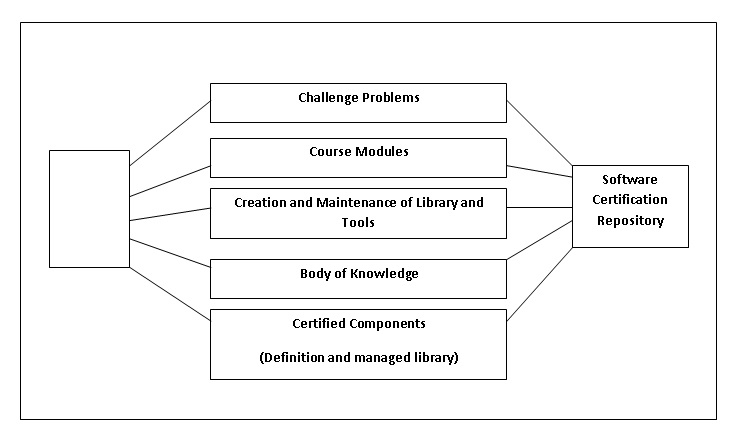
\includegraphics[width=110mm]{Images/Overview_SW_Repo.jpg}
\caption{Design of Software Repository}
\label{Fig:1}
\end{figure}


The repository would have a schema design for each of these components. The schema would be designed as XSD which would cover all the required parameters to store the required data for that component. The actual data is then stored in XML format after validating it against the corresponding XSD schema. Finally, XSLs designed according to respective schemas of the components of repository, are used to view XMLs  in the browser. 

This report considers first three components of this repository viz. Challenge Problems, Course Modules and Creation and Maintenance of Library and Tools. The Challenge Problem part of the repository is meant to store some challenge problems in the area of software certification. XMLs added to the repository would contain all the information regarding a particular challenge and would be created according to a general schema designed for challenge problems. Course modules intend to have all the information about the courses involving topics in software certification. This information is again in XML format following schema designed for Course Module component of Software Repository. The last component manages information about libraries and verification tools. Libraries comprises of two types. It can either be a library which is a part of a verification tool or it can be a library which is verified by a verification tool. XMLs representing libraries and tools are validated against two separate schemas for libraries and tools respectively. 

The subsequent chapters of the report documents the entire process of schema designing, XML and XSL creation and provide schemas, XSLs and some sample XMLs used for testing the corresponding schemas for above three parts of software repository.  

\chapter{Challenge Problems}

Challenge problems are sets of prototypes of problems in software certification area. The software repository intends to store all the available and relevant challenge problems. This includes both solved and unsolved challenge problems meaning that the solution is also saved if it is available. Challenge problems can be part of various conferences held for the software community. For example, there are challenges called SAT challenge, CADE ATP  challenge , Pacemaker challenge, SMT COMP challenge, SV-COMP challenge \cite{SAT,CADE,Pacemaker,SMT,SV} etc. have been offered as a part of various conferences and workshops. Each challenge has different dimensions. 

The requirements and specifications depend on the actual challenge problem and their organization meaning the committee who is putting forward this challenge. As the purpose of the repository is to collect all the challenge problems, a general schema which would be able to catch all the information of diverse challenge problems is needed. The schema provides a schematic structure to the repository in order to store challenge problems.  

\section{Schema Design} 
The first step in schema designing process is to analyze various challenge problems and try to find out some attributes which are common in all the challenges. The collective attributes actually are various the parameters in different challenges which make it possible to preserve their information in a structured manner. 

As specified earlier, the schema is designed using XSD. Thus, all the information is tracked in the form of tags using XMLs. The XMLs of various challenges are then validated against the same designed schema. The schema portrays the general structure for all the challenges still allowing users to embed challenge specific information in the XMLs. The Listing \ref{lst:attCP} shows all the attributes derived after analyzing some challenge problems.

\lstinputlisting[label=lst:attCP,escapeinside={@}{@},caption = {Attributes for Challenge Problem Schema}]{Code/AttributeListingChallengeProblem.txt}

\bigskip
Attributes' names indicate the purpose of the attribute. Thus, it covers all the required parameters regarding the challenge such as its name, area, its description, associated conference, rules to solve the challenge, documentation, tools allowed, expected solution format, available solutions, assessment details, deadlines and contacts. Some challenge problems also have a set of benchmark problems. Benchmark problems are smaller sets of problems related to main challenge problem. Their formats, rules and solutions vary from challenge to challenge. Some attributes are used to tag this important information about benchmarks as well. Therefore, this listing of attributes provides a hierarchical structure to tag information about various challenge problems and thus makes it convenient to implement this schema design using XSD.

\section{Implementation}
The above schema design is implemented using XSD. The whole schema is broken down into three schemas. The first one has all the elements common to the areas covered in this report meaning that it contains all the attributes common in the areas of challenge problems, course modules, libraries and tools. The second schema contains the elements required to tag detail information regarding execution environment. The third schema is the actual main schema for challenge problem which includes the above two schemas. An online tool is used to validate XMLs against this schema \cite{olXSD}.

\subsection{Common Schema}
As described earlier, this schema represents all the common attributes to the three areas covered in this report. This is done to avoid redundancy in implementing the entire schema. This schema would be included in all the main schemas for challenge problems, course modules, libraries and tools. The Listing \ref{lst:common} displays the code for the common schema.     

\lstinputlisting[label=lst:common,escapeinside={@}{@},caption = {Common Schema}]{Code/CommonSchema.txt}

\subsection{Schema for Execution Environment}
This schema represents particularly the information specific to execution environment for the challenge problems. It separates all the execution environment data from the other elements of challenge problems such as its description, assessment details, contacts etc. This schema stores data like expected solution format, libraries, compilers, processors and OS permissible to solve the challenge and basically all the elements needed to describe the expected solution as well as existing solutions. The Listing \ref{lst:ExEn} shows the code for Execution Environment Schema. 

\lstinputlisting[label=lst:ExEn,escapeinside={@}{@},caption = {Execution Environment Schema}]{Code/ExecutionEnvironmentSchema.txt}

\subsection{Challenge Problem Schema}
This is the main schema for challenge problems. The structure of the schema is according to the schema design described earlier. It includes the two supporting schemas viz. Common Schema and Execution Environment Schema explained in the above sub sections. The Listing \ref{lst:CPSchema} displays the code for challenge problem schema.

\lstinputlisting[label=lst:CPSchema,escapeinside={@}{@},caption = {Challenge Problem Schema}]{Code/ChallengeProblemSchema.txt}

\section{Viewing Data in Browser}
The data stored in the repository is in the form of XMLs which are validated against the above schema designed for Challenge Problems. Hence, some mechanism is needed to visualize those XMLs in the browser making them easy to interpret and read. This is done using XSLT. XSL is used to transform XML code into HTML code which is read by the browser and thus displays the contents of the XML file in the form of a html page. 

The XSL for challenge problem reads the contents from the XML files according to the challenge problem schema and displays the information in proper format if it is present in the XML file. An online tool is used to transform XML with XSL \cite{olXSL}. The tool accepts both the XML and XSL and then transforms XML code into HTML code understood by the browser. This html file is then viewed in the browser. Thus, XSL is used to display the data stored in the repository in readable format and hence is similar to the data retrieving process. The Listing \ref{lst:XSLCP} depicts some part of the code for XSL for challenge problems.

\lstinputlisting[label=lst:XSLCP,caption = {Sample of XSL for Challenge Problems}]{Code/XSLChallengeProblem.txt}

\bigskip
The testing of the above schemas and XSL along with a case study is described in detail later in the report. 

\chapter{Course Modules}
The software repository collects some course modules related to software certification area \cite{York,Waterloo,MaC,Victoria}. Thus, the main objective behind this schema designing process is to identify the essential elements in various courses offered in these areas. This provides a schematic structure in order to be able to tag all the information related to various courses. Some examples of course modules are courses related to safety critical systems, embedded systems and real time systems. Hence, relevant course modules are basically those which are related to some systems containing software configuration. 

\section{Schema Design}
Similar to challenge problem schema design, the first step here is again to analyze various course modules and figure out common elements. The elements altogether represent all the information of the course modules. Note that here the main focus is to collect all time independent data. Therefore, the major goal of analysis of various challenges is to find out attributes such as learning outcomes, aim of the module, pre-requisites and contents rather than focussing on deadlines and timings.  

This schema is also implemented using XSD. Thus, all the attributes found by analyzing various course modules are organized in a hierarchical structure making the translation to XSD easy. The Listing \ref{lst:attCM} shows all the attributes used to implement course module schema.

\lstinputlisting[label=lst:attCM,escapeinside={@}{@},caption = {Attributes for Course Modules Schema}]{Code/AttributeListingCourseModule.txt} 

\section{Implementation}
The schema implementation follows the schema discussed in above section. It also includes the common schema implemented given in Listing \ref{lst:common}. This schema again covers the general structure to tag all the attributes of course modules in diverse areas while allowing to save some module specific data as well. The schema is then tested with some sample course module XMLs by using an online XML schema validation tool \cite{olXSD}. The testing details are discussed later in the report.  The Listing \ref{lst:CMSchema} shows the code for course module schema.

\lstinputlisting[label=lst:CMSchema,escapeinside={@}{@},caption = {Course Module Schema}]{Code/CourseModuleSchema.txt} 

\section{Viewing Data in Browser}
Similar to challenge problems XMLs, course module XMLs also need a XSL to transform XML code into HTML code. This makes it able to be viewed in the browser. The XSL is implemented according to the course module schema given above. It checks if the information is present in the XML or not and then converts it into appropriate HTML code. The HTML code displays information in an eye pleasing and organized format. An online tool is used to transform XMLs using this XSL \cite{olXSL}. As discussed earlier, the tool accepts both XML and XSL, then transforms the given XML accroding to the XSL finally providing an HTML code as an output. The Listing \ref{lst:XSLCM} shows some sample of XSL code for course modules. 

\lstinputlisting[label=lst:XSLCM,caption = {Sample of XSL for Course Module}]{Code/XSLCourseModule.txt}

\bigskip

The testing of the XSL with some sample XMLs is done and is later discussed in the report. 

\chapter{Libraries and Tools}
The third component of the repository saves the data related to libraries and tools. The repository requires a schema to store some certified software libraries as well as some verification software tools used in the area of software certification. Libraries and tools are related to each other. Tools are referred as a certification mechanism for libraries. The report presents two separate schemas for libraries and tools respectively.   

\section{Schema Design}
The design process again begins with some sample libraries and tools \cite{Alea, DFC, MCHIP,COQ, CADP}. They are analyzed and attributes for the schemas are figured out. The schema for the library should be able to tag all the data related to a library such as its current versions, contents, downloading, tools used for compilation or verification, examples, references and dependencies if any. Along with these elements, some additional elements like execution environment, functionalities, getting the tool are added to the tools' schema. However, even though the tools and the libraries schemas contain some common elements they have their own attributes too and needs to be stored separately. Thus, they have their own attribute listings and implementations.
\subsection{Attributes Listing: Libraries}
The analysis of some libraries such as Microchip certified libraries, a COQ libraries and a PRL math library, some attributes regarding the libraries are noted down in hierarchical format. The Listing \ref{lst:attL} shows the elements for the libraries' schema.

\lstinputlisting[label=lst:attL,escapeinside={@}{@},caption = {Attributes for Libraries' Schema}]{Code/AttributeListingLibraries.txt} 

\subsection{Attributes Listing: Tools}
After analyzing some tools like COQ, CADP, NuSMv etc \cite{COQ,CADP}., some elements which constitute the tool's schema are found out.The Listing \ref{lst:attT} shows the elements for the tools' schema. 

\lstinputlisting[label=lst:attT,escapeinside={@}{@},caption = {Attributes for Tools' Schema}]{Code/AttributeListingTools.txt}  
\section{Implementation}
As mentioned earlier, libraries and tools are related to each other. So, naturally they share some common elements which can be implemented separately. Moreover, both of these schemas also include the common schema discussed earlier in Listing \ref{lst:common}. The latter chapter talks about the testing of these schemas in detail. 
\subsection{Common Schema for Libraries and Tools}
The schema mainly contains implementation of a few common elements such as version details, contents' details and extensions. The Listing \ref{lst:CSLT} shows the common schema code for libraries and tools.
\lstinputlisting[label=lst:CSLT,escapeinside={@}{@},caption = {Common Schema for Libraries and Tools}]{Code/CommonSchemaLibrariesTools.txt}  
\subsection{Schema for Libraries}
The Listing \ref{lst:SL} contains the implementation for libraries' schema. 
\lstinputlisting[label=lst:SL,escapeinside={@}{@},caption = {Schema for Libraries}]{Code/LibrariesSchema.txt}
\subsection{Schema for Tools}
The Listing \ref{lst:TL} gives the implementation for tools' schema. 
\lstinputlisting[label=lst:TL,escapeinside={@}{@},caption = {Schema for Libraries}]{Code/ToolsSchema.txt}

\section{View Data in Browser}
Similar to challenge problems and course modules, libraries and tools XMLs are viewed in the browser with the help of XSLs. 
\subsection{XSL for Libraries}
The Listing \ref{lst:XSLLib} shows some part of the XSL code for the libraries. 
\lstinputlisting[label=lst:XSLLib,caption = {Sample of XSL for Course Module}]{Code/XSLLibraries.txt}
\subsection{XSL for Tools}
The Listing \ref{lst:XSLTools} shows some part of the XSL code for the tools. 
\lstinputlisting[label=lst:XSLTools,caption = {Sample of XSL for Course Module}]{Code/XSLTools.txt}

\chapter{Testing}

The testing begins with preparing some sample XMLs for all the areas discussed. The whole schema design, implementation, XSLs implementation and testing process follows an iterative approach. All the three areas viz. challenge problem, course modules and Libraries and tools are tested individually. However, they follow the same testing process. 

\section{Test Cases}
After the schema design and implementation, a XML is prepared from a sample challenge problem, course module, library and a tool. This XML is validated against the first version of the schema. Some test cases described in table \ref{table:test} are tested to check the strength, validity and effectiveness of the schema. According to the results, improvements are made to the schema. This process is repeated till the schema is tested against reasonable number of samples and passes all the test cases correctly without the further need of modification to the existing schema. 

The set of XML samples is then transformed using the XSL designed according to the final tested schema. The HTML file produced as an output is tested against some test cases given in table \ref{table:test}. This again follows the iterative approach till all the test cases are satisfied.

The table \ref{table:test} lists down the test cases used for both XSDs and XSLs of challenge problems, course modules, libraries and tools.
%\thispagestyle{empty}
%\vspace*{-\baselineskip}
\begin{table}
\begin{tabular}{| l | p{2cm} | p{5cm} | p{2cm} | p{1cm} |}
\hline \textbf{Sr.No.} & \textbf{Test Case Name} & \textbf{Description} & \textbf{Applicable For} & \textbf{Result} \\ \hline 1. & Information coverage & check whether all the information is covered & XSD/XSL & Passed \\ 
\hline 2. & Appropriate attribute tagging & All the information should be tagged appropriately.  & XSD & Passed  \\  
\hline 3.& Allowance of specific information  & Specific but important information for the challenge should also be covered without affecting the general structure of the schema & XSD & Passed \\ 
\hline 4.& Flexibility & Not all the elements are present in all the samples. The schema should allow users to insert only available information. Checking the use of optional attributes. & XSD/XSL & Passed. \\ 
\hline 5. & Attribute coverage & Testing on reasonable number of samples to verify all the attributes in the schema or XSL are utilized & XSD/XSL & Passed \\  
\hline 6. & Common schema & Use of common schema to implement common elements & XSD & Passed \\  
\hline 7. & Look and feel for XSL & Checking whether all the information when viewed in the browser is properly aligned and look and feel of HTML page & XSL & Passed \\ 
\hline
\end{tabular}
\caption[Table caption text]{Test Cases}
\label{table:test}
\end{table}
\pagebreak
\section{Case Study}
This section gives a sample XML and its transformed HTML code for a challenge problem. The XMLs illustrate how the actual information is stored in the repository using the newly designed schemas and HTML files depict how the XMLs are transformed and viewed in the browser using the newly XSLs implemented according to the corresponding schemas. 

Note that the report just gives one sample XML and HTML for a challenge problem. However, the schemas and XSLs are tested against reasonable number of XMLs in order to verify their validity and effectiveness and similarly XMLs and HTMLs can be obtained for other categories and data samples.

Additionally, the XML and HTML has been truncated to fit inside the report. The actual files are longer than the ones included in the report. Thus, they act like representatives for all the XMLs and HTMLs required.

The Listing \ref{lst:XMLSAT} gives XML for SAT challenge. The XML is prepared by extracting the information from SAT challenge website and then tagging it according to the challenge problem schema given in the Listing \ref{lst:CPSchema} \cite{SAT}. The XML is then validated using the online tool against the challenge problem schema \cite{olXSD}. 

\lstinputlisting[label=lst:XMLSAT,caption = {Sample XML for Challenge Problems: SAT Challenge}]{Code/XMLSatChallenge.txt}

\bigskip
The Listing \ref{lst:HTMLSAT} gives the HTML code for above XML after transforming it using the corresponding XSL with the help of a tool \cite{olXSL}.

\lstinputlisting[label=lst:HTMLSAT,caption = {Sample HTML for Challenge Problems: SAT Challenge}]{Code/HTMLSAT.txt}

\chapter{Conclusion}
Software certification refers to the process of certification of software part in the system. The report talked about some approaches to accomplish this. Component reusability is now getting popular in software certification. However, the component to be reused needs to have the appropriate certification and certification management system. One of the challenges in this area is the management of useful information regarding the certification. Therefore, the report proposed the overall design of the software repository which would manage information related to various areas around software certification, mainly focussing on the three areas viz. challenge problems, course modules and libraries and tools. 

Future tasks for the repository can be categorized into two streams. First one would be to find more samples for all the three components discussed here. The major challenge for the work presented in the report was data gathering. It is a challenging task to find the relevant data samples. This is true for all the areas such as challenge problems, course modules, libraries and tools. Hence, the next task for the three areas in the report is to find some more relevant challenge problems, course modules, libraries and tools. The second part of the future task is to design and implement schema for the rest of the two areas of the repository. The schemas can be designed and implemented by following the same methods illustrated in the report. This would complete the implementation of the proposed repository. 

Finally, to conclude, the report explained the process of schema designing and presented implementations followed by their XSL implementations for the three areas such as challenge problems, course modules, libraries and tools related to software certification and therefore provided an effective mechanism to index some available materials around these areas. 

\bibliographystyle{alpha}
\bibliography{References_Report_Ishwaree_Argade}

\end{document}